% The \documentclass command is the first command in a LaTeX file.
% \documentclass{bsu-ms}
\documentclass[project,Amit]{bsu-ms}  % for project reports

%%%%%%%%%%%%%%%%%%%%%%%%%%%%%%%%%%%%%%%%%%%%%%%%%%%%%%%%%%%%%%%%%%%%%%%%%%%%%%
% Packages

% The 'graphicx' package is quite extensive; the main purpose here is
% the includion of PostScript graphics.  The 'dvips' option makes it work
% better with 'dvips' (which is what is often used under Linux)
\usepackage[pdftex]{graphicx}

% The 'ulem' package is used to underline with dotted or dashed line.
\usepackage[normalem]{ulem}
\def\dotuline{\bgroup 
  \ifdim\ULdepth=\maxdimen  % Set depth based on font, if not set already
   \settodepth\ULdepth{(j}\advance\ULdepth.4pt\fi
  \markoverwith{\begingroup
  \advance\ULdepth0.08ex
  \lower\ULdepth\hbox{\kern.15em .\kern.1em}%
  \endgroup}\ULon}
\def\dashuline{\bgroup 
  \ifdim\ULdepth=\maxdimen  % Set depth based on font, if not set already
   \settodepth\ULdepth{(j}\advance\ULdepth.2pt\fi
  \markoverwith{\kern.10em
  \vtop{\kern\ULdepth \hrule width .2em}%
  \kern.10em}\ULon}

% The 'subfigure' package does a nice job handling and labelling subfigures
\usepackage{subfig}
\usepackage{url}
\usepackage{citesort}

\usepackage{enumitem}
\setlist{nolistsep}

%%%%%%%%%%%%%%%%%%%%%%%%%%%%%%%%%%%%%%%%%%%%%%%%%%%%%%%%%%%%%%%%%%%%%%%%%%%%%%
% Local commands

% Define your macros (new commands) here.


%%%%%%%%%%%%%%%%%%%%%%%%%%%%%%%%%%%%%%%%%%%%%%%%%%%%%%%%%%%%%%%%%%%%%%%%%%%%%%
% Front Matter Definitions
%%%%%%%%%%%%%%%%%%%%%%%%%%%%%%%%%%%%%%%%%%%%%%%%%%%%%%%%%%%%%%%%%%%%%%%%%%%%%%

% These definitions are used by the commands below to construct the front 
% matter pages.  

% Document title
% The \titleBreak command produces a line break in the title on the
% title page (this may be necessary to keep longer titles from looking
% strange)
\title{Hadoop and Hive as Scalable alternatives to RDBMS: A Case Study}  
\author{Marissa Rae Hollingsworth}  

\graduationDay{13}
\graduationMonth{August}
\graduationYear{2012} 

\advisor{Amit Jain} % also the chair of your committee
\committeeA{Murali Medidi} 
\committeeB{Jyh-haw Yeh}
\degree{Master of Science}
\major{Computer Science}
\department{Computer Science}
\college{Engineering}
\departmentChair{Murali Medidi}
\graduateDean{John R. Pelton}

\abstract
{ 
While high-performance, cost-effective data management solutions, such as Hadoop, exist for Big Data analysis, small and medium businesses with moderate-sized data sets would also like to implement low budget data management systems that will perform well on existing data and scale as the amount of accumulated data increases. Parallel database management systems may provide a high-performance solution, but are expensive and complex to implement. The purpose of this project was to compare the scalability of open-source relational database management systems and distributed data management systems for small and medium data sets. To make this comparison, a business intelligence case study was investigated using three data management solutions: MySQL, Hadoop MapReduce, and Hive. This experiment involved a payment history analysis which considers customer, account, and transaction data for predictive analytics. Experiments were executed on data sets ranging from 200MB to 10GB. The results show that the single server MySQL solution performs best for trial sizes ranging from 200MB to 1GB, but does not scale well beyond that. MapReduce outperforms MySQL on data sets larger than 1GB and Hive outperforms MySQL on sets larger than 2GB. This demonstrates MapReduce and Hive as viable techniques for small and medium businesses who want to implement scalable data management techniques.
}

\includeCopyright

\maxPage{199}

\acknowledgments{
I would like to thank my advisor, Dr. Amit Jain, for the dedication and encouragement he gave during both my undergraduate and graduate studies at Boise State University. I would also like to thank my committee members, Dr. Murali Medidi and Dr. Jyh-haw Yeh, Dave Arnett and Vince Martino for the guidance they provided. And finally, I would like to thank my family and friends for their encouragement, love and support; I could not have done this without them. 
}

\dedication{
For Nathan.
}

\biosketch{
Marissa Hollingsworth was born in Carlsbad, California and moved to Boise, Idaho in 2004. She graduated from Skyview High School in 2004 and attended Boise State University for her undergraduate career. She graduated from Boise State with a Bachelor of Science degree in Computer Science in 2009 and began her graduate studies at Boise State University immediately after, working as a graduate teaching assistant for the computer science department. In June of 2011, she began her career as a Software Design Engineer at HP Indigo in Boise, where she is currently employed.
}

% (End of preamble)
%%%%%%%%%%%%%%%%%%%%%%%%%%%%%%%%%%%%%%%%%%%%%%%%%%%%%%%%%%%%%%%%%%%%%%%%%%%%%%

\begin{document}
\frontmatter  %! Do not remove! 
\buildFrontPages %! Do not remove! 

% The (optional) list of abbreviations goes here
% \begin{listAbbreviations}
%   \item[RDBMS] Relational Database Management System
% \end{listAbbreviations}

% The (optional) list of symbols goes here
% \begin{listSymbols}
%   \item[$\sqrt{2}$] square root of 2
%   \item[$\lambda$] lambda symbol, normally used in lambda calculus but
%     it sometimes gets used for wavelength as well
% \end{listSymbols}

\mainmatter

%%%%%%%%%%%%%%%%%%%%%%%%%%%%%%%%%%%%%%%%%%%%%%%%%%%%%%%%%%%%%%%%%%%%%%%%%%%%%%
%
% Chapter: Introduction
%
%%%%%%%%%%%%%%%%%%%%%%%%%%%%%%%%%%%%%%%%%%%%%%%%%%%%%%%%%%%%%%%%%%%%%%%%%%%%%%
%%%%%%%%%%%%%%%%%%%%%%%%%%%%%%%%%%%%%%%%%%%%%%%%%%%%%%%%%%%%%%%%%%%%%%%%%%%%%%
%
% Chapter: Introduction
%
%%%%%%%%%%%%%%%%%%%%%%%%%%%%%%%%%%%%%%%%%%%%%%%%%%%%%%%%%%%%%%%%%%%%%%%%%%%%%%
\chapter{Introduction} \label{ch:intro}
\section{Overview}
The persistent evolution of digital technology is unlocking new forms of Business Intelligence (BI). The acquisition, storage, access, and analysis of digital information provides knowledge and strategic insights for enterprise and research organizations. Each time we visit a website or make a transaction, the owner has the ability to log everything we do; every link we click, each form we submit, what time we log in and out, any errors we encounter, and just about anything else we can imagine. While this information may seem useless and doesn't appear to affect the user much, the site owner now has valuable information that can give him or her the competitive advantage. The collected data can be stored in log files and analyzed for BI that can be used to develop and incorporate new business strategies and direct planning for the future.

In terms of BI data management, collection is generally the easy part-- it is the storage and access aspects (requisites for later BI analytics) that impose major challenges for \textit{small and medium businesses} (SMB)-- especially since data can accumulate to gigabytes and even terabytes in a relatively short period of time. Thus, data management becomes a greater obstacle as more and more data needs to be collected and stored. Traditionally, businesses have been able to store their data in local data centers comprised of a few machines. However, as data outgrows the capacity of local data centers, they must modify their storage methods. Even if the company expands the data to multiple machines, they must develop ways of accessing the data. In BI, more data reveals new doors and opportunities for the organization in terms of derived knowledge and achieving a competitive advantage, but the information is effectively useless if they can't consider all of it simultaneously in their strategic analysis.

Providing a multi-layer model of staging, integration, and access to historical data archives is fundamental to BI for any modern organization. Staging is used to store raw data for use by developers, integration is used to incorporate data into the storage system while maintaining a level of abstraction from users, and the access layer is for getting data out for the end users. Due to the sensitive and irreplaceable nature of customer data, enterprise storage systems must provide data replication, backup and recovery, data integrity, and concurrency control. Common storage systems include data transformation algorithms to transform data to the correct format. The system interacts with the operating system to send the data from the user to the storage system. There are several database management systems which conform to these requirements, but the most popular is the \textit{relational database management system} (RDBMS). 

As the size of data sets increase, it is possible to run out of space on a single system. When this happens, the data may be moved to a parallel RDBMS or distributed among several networked systems and managed by a \textit{distributed data management system} (DDMS). Parallel RDBMSs have been commercially available for several decades and offer high performance and high availability for data management. However, the up-front costs and the cost to scale up for larger storage capacities can be expensive. On the other hand, freely available DDMSs offer high performance and high availability, but at much lower up-front and scaling costs.  

In this research, we investigate the performance of \textit{open-source software} (OSS) solutions on mid-sized data sets for SMBs using a realistic case study. We conduct this experiment between a RDBMS, namely MySQL, and a DDMS, namely Hadoop, which is a resource-effective solution for SMBs. We investigate MapReduce and Hive as two techniques for analyzing the data stored in Hadoop.

\section{Structure}
In Chapter~\ref{ch:background} we provide the background for concepts pertaining to BI storage, access, and analytical systems. Here, we outline some challenges faced by SMBs interested in BI analytics and discuss RDBMS and alternative DDMS solutions. We summarize the notion of Big Data, a likely future obstacle for the SMB, and provide relevant information regarding the Hadoop solutions considered in this research: MapReduce and Hive.

In Chapter~\ref{ch:problem} we introduce the payment history analysis case study for a specific SMB. This particular SMB designs software tools to analyze current and historical payment habits on customer data and attempts to forecast trends. We discuss the database management challenges faced by the SMB as their customer base expands and define their specific case study. Here, we explain their data storage and access models, along with the requisite test data set generation utilities required to conduct the analysis. In doing so, we formally present the problem statement and list the inquiries we wish to address in this research project.

In Chapter~\ref{ch:solution} we define the design and implementation for the RDBMS and DDMS solutions. First, we discuss the detailed process of generating the test data set and provide a summarized description of the key algorithms and data structures employed by these utilities: the \texttt{HistogramGen} and \texttt{AccountGen} MapReduce programs. Second, we discuss the central components of the MySQL, Hadoop MapReduce, and Hadoop Hive solution implementation, where we explain the process by which they are used to instrument the payment history analysis case study (as presented in Chapter~\ref{ch:problem}).

In Chapter~\ref{ch:results} we detail the RDBMS and DDMS performance comparison experiment (for the solutions from Chapter~\ref{ch:solution}). Here, we discuss the efficiency and scalability for these implementations, along with the resulting implications and analysis for this SMB's data management case study (as expressed in Chapter~\ref{ch:problem}). First, we discuss the software and hardware environment in which our comparative benchmark analysis is conducted. Second, we provide the procedure used to guide and execute the experiment. Finally, we present the performance results for the various experimental trial runs.

In Chapter~\ref{ch:conclusion} we conclude our report and suggest some future directions.
%%%%%%%%%%%%%%%%%%%%%%%%%%%%%%%%%%%%%%%%%%%%%%%%%%%%%%%%%%%%%%%%%%%%%%%%%%%%%%%
%
% Chapter: Business Intelligence and Data Warehousing
%
%%%%%%%%%%%%%%%%%%%%%%%%%%%%%%%%%%%%%%%%%%%%%%%%%%%%%%%%%%%%%%%%%%%%%%%%%%%%%%%
%%%%%%%%%%%%%%%%%%%%%%%%%%%%%%%%%%%%%%%%%%%%%%%%%%%%%%%%%%%%%%%%%%%%%%%%%%%%%%
%
% Chapter: Business Intelligence and Data Warehousing
%
%%%%%%%%%%%%%%%%%%%%%%%%%%%%%%%%%%%%%%%%%%%%%%%%%%%%%%%%%%%%%%%%%%%%%%%%%%%%%%
\chapter{Background}\label{ch:background}
\section{Business Intelligence}
BI aims to support decision-making for an organization. As digital information becomes more prevalent, service providers are seeking guidance as to how they can leverage the data they collect to improve their knowledge base for incorporating new strategies into their business. BI technologies provide historical, current and predictive views of business operations; BI software is designed to perform a wide variety of such functions, ranging from online analytical processing, to business performance management, to data, process, and text mining. 

Until recently, the focus for data analysis had been on large enterprises with vast amounts of data. However, a major problem faced by SMBs in today's economy is their lack of management expertise and financial reporting that investors need to make decisions about whether or not to invest \cite{Newberry}. More than one-quarter of SMBs indicated that ``getting better insights from the data'' they have is a top technology challenge \cite{smbroutes}. Overcoming this mode of challenges places crucial importance on the ability to implement a scalable BI solution based on the available data and thereby provide a means to acquire valuable insights into business trends.

In general, a BI system comprises three essential and distinct components, namely \textit{data sources}, \textit{data warehousing}, and \textit{analytics}. Data may be sourced from a diverse set of entities, which may be external (i.e. industry reports, media data, business partners, etc.) and/or internal (i.e. account transactions, employee reports, client reports, etc.). Data sets used for BI is typically defined as Big Data and may be unstructured and complex. Data warehousing is essential to an effective BI system and should be disjoint from the operational data storage required for day-to-day business operations. In this context, a data warehouse contains a historical data store designed to manage data accumulated over time and an analytical data store designed to manage and make available a subset of the historical store for predictive analysis. Finally, the analytics component includes the software tools which access the analytical data store and instrument the prediction procedure(s).

In the initial BI development stages it is typical for businesses to use a RDBMS for \textit{both} operational and data warehousing. When the data sets are small, this strategy is beneficial because the approach is relatively simple, efficient, and cost-effective. However, as time progresses and accumulated data increases, this ``one size fits all'' approach does not work well with BI analysis, largely due to the underlying architecture of the database~\cite{stonebraker,jacobs2009pathologies}. ``To achieve acceptable performance for highly order-dependent queries on truly large data, one must be willing to consider abandoning the purely relational database model for one that recognizes the concept of inherent ordering of data down to the implementation level''~\cite{jacobs2009pathologies}. Distributed solutions designed to manage big data, such as the Apache Hadoop project, are adopted to meet these new requirements. The following sections provide background information on the RDBMS and big data analysis techniques used in our research-- MySQL and Apache Hadoop, respectively.

\section{Relational Database Management Systems}
The relational database is the most popular database model used for the storage and access of operational data that is optimized for real-time queries on relatively small data sets. Data is organized as a set of formally-described tables whose fields are represented as columns and records are represented as rows in the table~\cite{codd1970relational}. A RDBMS is the software which controls the storage, retrieval, deletion, security, and integrity of data within a relational database~\cite{amblers}. Data can be accessed and reassembled in several ways for both interactive queries and gathering data for reports via structured query language (SQL) operations based on relational algebra.

\subsection{MySQL}
MySQL Community Edition is the free version of ``the world's most popular'' open-source RDBMS implementations that is supported by a huge and active community of open source developers. MySQL supports many standard DBMS features including replication, partitioning, stored procedures, views, MySQL Connectors for building applications in multiple languages, and the MySQL Workbench for visual modeling, SQL development and administration~\cite{mysql}. Many organizations such as Facebook, Google, Adobe, and Zappos use MySQL to power high-volume web sites, business-critical systems and packaged software.

A typical MySQL deployment includes a server installed on a single, high-end server which accepts local and remote client queries. Since the database is limited to the hard drives of the server, when the amount of data exceeds the limited storage capacity, this model will fail and a DBMS with an underlying distributed storage system will need to be employed.
%===============================================================================
% Section: Distributed: Apache Hadoop
%===============================================================================
\section{Big Data Analytics}
While the RDBMS model is well suited and optimized for real-time queries on relatively small data sets, it was \textit{not} designed for Big Data analysis, largely due to the limited storage capacities and the underlying write-optimized ``row-store'' architecture~\cite{stonebraker}. While write-optimization allows for efficient data import and updates, the design limits the achievable performance of historical data analysis that requires optimized read access for large amounts of data. Another drawback of the RDBMS approach stems from the lack of scalability as the number of stored records expands. To overcome this obstacle, we can move data to a parallel DBMS system. 

Parallel DBMSs share the same capabilities as traditional RDMBSs, but run on a cluster of commodity systems where the distribution of data is transparent to the end user~\cite{pavlo}. Parallel RDBMSs have been commercially available for several decades and offer high performance and high availability, but are much more expensive than single-node RDBMSs because there are no freely available implementations and they have much higher up-front costs in terms of hardware, installation, and configuration~\cite{stonebraker2010mapreduce}. In contrast, Hadoop can can be deployed on a cluster of low-end systems and provides a cost-effective, ``out-of-the-box'' solution for Big Data analysis.  While some parallel DBMSs may have relative performance advantages over open-source systems, such as Hadoop, the set-up cost and cost to scale may deter SMBs from using them. Furthermore, Hadoop is better suited for BI analysis because it allows for the storage and analysis of unstructured data, while parallel DBMSs force the user to define a database schema for structured data~\cite{pavlo}.

\subsection{Hadoop Distributed Filesystem}
Hadoop is an open-source Java implementation of the MapReduce framework developed by Google. The Apache Software Foundation and Yahoo! released the
first version in 2004 and continue to extend the framework with new sub-projects. Hadoop provides several open-source projects for reliable, scalable, and distributed computing~\cite{hadoop}. Our project will use the Hadoop Distributed Filesystem (HDFS)~\cite{hdfs}, Hadoop MapReduce~\cite{mapreduce}, and Hive~\cite{hive}.

The Hadoop Distributed Filesystem (HDFS) is a scalable distributed filesystem that provides high-throughput access to application data~\cite{hdfs}. HDFS is written in the Java programming language. A HDFS cluster operates in a master-slave pattern, consisting of a master \textit{namenode} and any number of slave \textit{datanodes}. The namenode is responsible for managing the filesystem tree, the metadata for all the files and directories stored in the tree, and the locations of all blocks stored on the datanodes. Datanodes are responsible for storing and retrieving blocks when the namenode or clients request them.

\subsection{MapReduce}\label{sec:mapreduce}
MapReduce is a programming model on top of HDFS for processing and generating large data sets which was developed as an abstraction of the \textit{map} and \textit{reduce} primitives present in many functional languages~\cite{mapreduce,Dean:2008:MSD:1327452.1327492}.  The abstraction of parallelization, fault tolerance, data distribution and load balancing allows users to parallelize large computations easily. The map and reduce model works well for Big Data analysis because it is inherently parallel and can easily handle data sets spanning across multiple machines.

Each MapReduce program runs in two main phases: the map phase followed by the reduce phase. The programmer simply defines the functions for each phase and Hadoop handles the data aggregation, sorting, and message passing between nodes.There can be multiple map and reduce phases in a single data analysis
program with possible dependencies between them. 
\begin{description}
 \item[Map Phase.] The input to the map phase is the raw data. A map function
should prepare the data for input to the reducer by mapping the key to the the
value for each ``line'' of input. The key-value pairs output by the map function
are sorted and grouped by key before being sent to the reduce phase. 
 \item[Reduce Phase.] The input to the reduce phase is the output from the map
phase, where the value is an iterable list of the values with matching keys.
The reduce function should iterate through the list and perform some operation
on the data before outputting the final result. 
 \end{description}

%-------------------------------------------------------------------------------
% Subsection: Hive
%-------------------------------------------------------------------------------
\subsection{Hive}
While the MapReduce framework provides scalability and low-level flexibility to run complex jobs on large data sets, it may take several hours or even days to implement a single MapReduce job~\cite{thusoo}. Recognizing this, Facebook developed Hive based on familiar concepts of tables, columns and partitions, providing a high-level query tool for accessing data from their existing Hadoop warehouses~\cite{thusoo}.  The result is a data warehouse layer built on top of Hadoop that allows for querying and managing structured data using a familiar SQL-like query language, HiveQL, and optional custom MapReduce scripts that may be plugged into queries~\cite{hive,thusoo2}. Hive converts HiveQL transformations to a series of MapReduce jobs and HDFS operations and applies several optimizations during the compilation process. 

The Hive data model is organized into \textit{tables}, \textit{partitions} and \textit{buckets}. The \textit{tables} are similar to RDBMS tables and each corresponds to an HDFS directory. Each table can be divided into \textit{partition}s that correspond to sub-directories within an HDFS table directory and each partition can be further divided into \textit{buckets} which are stored as files within the HDFS directories~\cite{thusoo2}. 

It is important to note that Hive was designed for scalability, extensibility, and batch job handling, \textit{not} for low latency performance or real-time queries. Hive query response times for even the smallest jobs can be of the order of several minutes and for larger jobs, may be on the order of several hours~\cite{hive}.
%%%%%%%%%%%%%%%%%%%%%%%%%%%%%%%%%%%%%%%%%%%%%%%%%%%%%%%%%%%%%%%%%%%%%%%%%%%%%%
%
% Chapter: Case Study: Payment Analysis for Business Intelligence
%
%%%%%%%%%%%%%%%%%%%%%%%%%%%%%%%%%%%%%%%%%%%%%%%%%%%%%%%%%%%%%%%%%%%%%%%%%%%%%%
%%%%%%%%%%%%%%%%%%%%%%%%%%%%%%%%%%%%%%%%%%%%%%%%%%%%%%%%%%%%%%%%%%%%%%%%%%%%%%%%
%
% Chapter: Case Study: Payment Analysis For Business Intelligence
%
%%%%%%%%%%%%%%%%%%%%%%%%%%%%%%%%%%%%%%%%%%%%%%%%%%%%%%%%%%%%%%%%%%%%%%%%%%%%%%%%
\chapter{Payment History Analysis: A Case Study and Problem Statement} \label{ch:problem}
The payment history analysis case study has been provided by a local software company who wishes to remain anonymous. From this point on, we will 
refer to this company as ``CompanyX''.  CompanyX provides software tools for customer information management and record analysis for BI. CompanyX evaluates current and historical payment habits for each customer account and attempts to predict future payment patterns based on past trends. Successful prediction of whether a payment will be on-time, past-due, or delinquent may reduce administrative costs accrued by outsourcing delinquent accounts for payment collection.  For example, if a customer has always made late payments in the past, they can expect that the customer will continue to make payments, even if they are late, and thus avoid sending them to a collection agency. 

As they expand their services, CompanyX expects the number of customers to increase from several hundred to several \textit{thousand}. This is a major cause for concern because the amount and complexity of collected data will increase as well, forcing the storage and access of data from their current hardware system to a more sophisticated system. Adopting a new hardware system while maintaining their existing service can be expensive, time-consuming, and may compromise data integrity and service availability as data is transferred from the old system to the new. Because of the risks involved, the company would like to compare the viability of other systems before converting their entire business architecture. This project will address the two major concerns that arise as a consequence of the increasing data volume: \textit{data storage model} and the \textit{scalability of data analysis software}. Due to privacy rights, any records collected by the company cannot be used, so sample data sets must be generated as prerequisite for testing new system implementations.

Our research assesses potential open source data warehousing models for CompanyX.

\section{The Case Study}

\subsection{Data Storage and Relationship Model}
The data must be staged for data warehousing. During this process, the data is pruned and normalized to fit a chosen data storage model. In this case, CompanyX has selected an RDBMS for data management (deployed on a local, in-house server), which is used for both operational and warehousing purposes. For this, the data is normalized to include a(n):
\begin{enumerate}
 \item \texttt{Customer} tuple for each customer (Table~\ref{tbl:custtuple}),
 \item \texttt{Account} tuple for each customer account (Table~\ref{tbl:accttuple}),
 \item \texttt{Transaction} tuple for each account transaction (Table~\ref{tbl:trantuple}), and
 \item \texttt{StrategyHistory} tuple for each account strategy (Table~\ref{tbl:strategytuple}).
\end{enumerate}
Note that the referenced tables use a solid underline to identify the \underline{primary key} and a dashed underline to identify a \dashuline{foreign key}. The relationship model between the tables is described below and shown in Figure~\ref{fig:eer-model}. 
%-------------------------------------------------------------------------------
% List of databaset tables
%-------------------------------------------------------------------------------
\begin{description}
 %------------------------------------------------------------------------------
 % Customer Tuple
 %------------------------------------------------------------------------------
 \item [Customer:]
  The unique \textit{primary key} for the customer entity-type is the
  \texttt{CustomerNumber} attribute. Each customer entity stores the
  customer's social security number (\texttt{ssn}) and the first three digits
  of the customer's zip code (\texttt{zipcode3}).
  \begin{table}[ht]
  \caption{ Customer Tuple }
  \label{tbl:custtuple}
  \centerline{
  \begin{tabular}{|l|l|l|l|l|}
   \hline
   \underline{CustomerNumber} & FirstName & LastName & Ssn & ZipCode3 \\
   \hline
  \end{tabular}
  }
 \end{table}
 %------------------------------------------------------------------------------
 % Account Tuple
 %------------------------------------------------------------------------------
 \item [Account:] 
  The unique \textit{primary key} for the account entity-type is the \texttt{AccountNumber} attribute. Each account entity includes the date the account was opened (\texttt{opendate}) and is \textit{is-owned-by} a unique customer, which is referenced by a foreign key\\ (\texttt{CustomerNumber}).
 \begin{table}[ht]
  \caption{ Account Tuple }
  \label{tbl:accttuple}
  \centerline{
  \begin{tabular}{|l|l|l|}
   \hline
   \underline{AccountNumber} & OpenDate & \dashuline{CustomerNumber}\\
   \hline
  \end{tabular}
  }
 \end{table}
 %------------------------------------------------------------------------------
 % Transaction Tuple
 %------------------------------------------------------------------------------
 \item [Transaction:]
The transaction entity is a weak type which depends on the account entity. Each transaction entity \textit{is-owned-by} a unique account which is referenced by the \texttt{AccountNumber} key and includes the type of transaction (\texttt{TransactionType} $\in$ \{\texttt{charge}, \texttt{adjustment}, \texttt{payment}\}), the date of the transaction (\texttt{TransactionDate}), and the amount of the transaction (\texttt{TransactionAmount}). The unique identifier is a \textit{composite key} composed of the \texttt{AccountNumber} reference, \texttt{TransactionType}, \texttt{TransactionDate}, and \texttt{TransactionAmount}.
 \begin{table}[ht]
  \caption{ Transaction Tuple }
  \label{tbl:trantuple}
  \centerline{
  \begin{tabular}{|l|l|l|l|}
   \hline
   \underline{\dashuline{AccountNumber}} & \underline{TransactionType} &
   \underline{TransactionDate}& \underline{TransactionAmount}\\
   \hline
  \end{tabular}
  }
 \end{table}
 %------------------------------------------------------------------------------
 % StrategyHistory Tuple
 %------------------------------------------------------------------------------
 \item [StrategyHistory:]
  The strategy history entity-type also depends on the account entity. Each
  strategy history entity \textit{is-owned-by} a unique account which is
  referenced by the \texttt{AccountNumber} key and includes the name of the strategy (\texttt{StrategyName} $\in$ \{\texttt{Good
  Standing}, \texttt{Bad Debt}\}) and the start date of the strategy
  (\texttt{StrategyStartDate}). The unique identifier is a \textit{composite key} composed of the \texttt{AccountNumber}
  reference, \texttt{StrategyName}, and \texttt{StrategyStartDate}.
 \begin{table}[ht]
  \caption{ StrategyHistory Tuple }
  \label{tbl:strategytuple}
  \centerline{
  \begin{tabular}{|l|l|l|}
   \hline
   \underline{\dashuline{AccountNumber}} & \underline{StrategyName} &
   \underline{StrategyStartDate}\\ 
   \hline
  \end{tabular}
  }
 \end{table}
\end{description}

%-------------------------------------------------------------------------------
% PaymentAnalysis Schema
%-------------------------------------------------------------------------------
\begin{figure}[ht]
\begin{center}
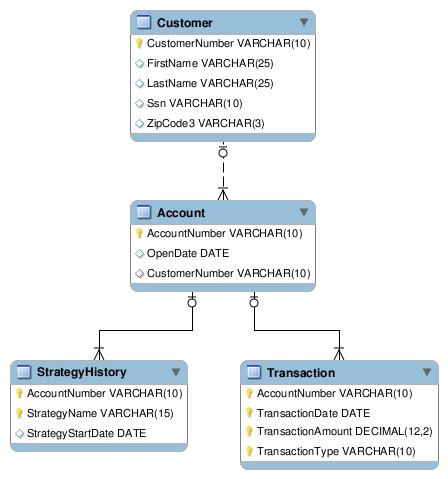
\includegraphics[width=\textwidth]{../images/account-history-schema.jpg}
\end{center}
\caption{Account history data entity-relationship model}
\label{fig:eer-model}
\end{figure}

\subsection{Data Access Model}
In order for CompanyX to use the data as input for their payment prediction algorithms, they must extract and prepare \textit{meaningful} data from the database. Data retrieval is achieved through join, aggregate, and other relevant SQL queries to the database. The resulting output of these queries must supply the input parameters for the prediction algorithms:
\begin{itemize}
 \item Aggregate charge, adjustment, and payment sums of historical transaction data.
 \item Aggregate payment sums of historical transaction data for all previous accounts owned by the same customer.
\end{itemize}

For a complete summary of CompanyX's expected output see Table~\ref{tbl:histtuple}.
{
\small
\begin{table}[ht]
 \caption{ Expected Result Tuple - Attribute descriptions }
 \label{tbl:histtuple}
 \centerline{
 \begin{tabular}{|l|p{7.5cm}|}
  \hline
  \textit{AccountNumber} & unique Account identifier\\ 
  \hline  
  \textit{OpenDate} & date the Account was opened by Customer\\
  \hline  
  \textit{ZipCode3} & first three digits of Customer's zip code\\
  \hline
  \textit{TotalCharges} & sum of all Charge transactions on Account\\
  \hline  
  \textit{TotalAdjustments} & sum of all Adjustment transactions on Account\\
  \hline
  \textit{AdjustedTotalCharges} & sum of TotalCharges and TotalAdjustments\\
  \hline
  \textit{TotalGoodStandingPayments30Day} & negative of sum of all payment
  transactions on account between 1 and 30 days after Good Standing strategy
  start date but before Bad Debt strategy start date\\
  \hline
  \textit{TotalGoodStandingPayments60Day} & same as above, but between 1 and 60
  days\\
  \hline
  \textit{TotalGoodStandingPayments90Day} & same as above, but between 1 and 90
  days\\
  \hline
  \textit{BadDebtTransferBalance} & sum of all transactions on account up
  through "Bad Debt" strategy start date\\
  \hline
  \textit{TotalBadDebtPayments30Day} & negative sum of all payment transactions
  on account between 1 and 30 days after Bad Debt strategy start date\\
  \hline
  \textit{TotalBadDebtPayments60Day} & same as above, but between 1 and 60
  days\\
  \hline
  \textit{TotalBadDebtPayments90Day} & same as above, but between 1 and 90
  days\\
  \hline
  \textit{PreviousAccountCount} & number of accounts with open date prior to
  this account's open date which have a customer with the same SSN\\
  \hline  
  \textit{PreviousAccountGoodStandingCharges} & sum of all charge transactions
  occurring prior to this account's open date on accounts which have a
  customer with the same SSN (not same account) which occurred while other
  accounts were at or after Good Standing strategy start date but before
  other accounts were at Bad Debt strategy start date\\
  \hline
  \textit{PreviousAccountGoodStandingAdjustments} & sum of all adjustments that
  occurred during Good Standing strategy for past accounts\\
  \hline
  \textit{PreviousAccountGoodStandingPayments} & sum of all Payments that
  occurred during Good Standing strategy for past accounts\\
  \hline
  \textit{PreviousAccountBadDebtPayments} & sum of all Payments that occurred
  during Bad Debt strategy for past accounts\\	
   \hline
  \end{tabular}
  }
 \end{table}
}

The first step of the retrieval process is to gather the transaction history data for each account, per strategy period. Recall that the relationships between account and transaction and customer and account are of \textit{one-to-many}. The total charges and adjustments do not depend on the strategy period, so these fields only require data stored in the \texttt{Transaction} table. However, because the account payments are subdivided into thirty, sixty and ninety day good standing and bad debt strategy periods, both the \texttt{StrategyHistory} and \texttt{Transaction} tables are required to select transactions per period. The process can be broken into these simplified steps:
\begin{enumerate}
 \item Join the \texttt{Account} and \texttt{Customer} tables to associate customer data with each account.
 \item Join the \texttt{Account} and \texttt{Transaction} tables to collect aggregate sums of \texttt{charge} and \texttt{adjustment} transactions, per account.
 \item Join the \texttt{Account}, \texttt{StrategyHistory} and \texttt{Transaction} tables to collect aggregate sums of \texttt{payment} transactions by strategy history type.
\end{enumerate}

At this point, the attributes stored in the result entity for an account include the customer data, total charges and adjustments, and payments per
strategy period. The next step will aggregate the transactions for all previous accounts with the same \texttt{ssn}. The result depends on the \texttt{OpenDate} of each account with the same \texttt{CustomerNumber} to determine if it is a previous account. If the account was opened before the
current account, then the result will depend on the \texttt{Transaction} and \texttt{StrategyHistory} tables. The process can be broken into these simplified steps:
\begin{enumerate}
 \item Determine the \texttt{ssn} of each account by joining \texttt{Account} and \texttt{Customer}.
 \item Left outer join \texttt{Account} table with itself on \texttt{ssn} and select accounts where \texttt{OpenDate} of the joined account is before the \texttt{OpenDate} of the left outer account.
 \item Join the result of the previous step with \texttt{StrategyHistory} and \texttt{Transaction} tables to collect aggregate sums of previous account
  transactions by transaction type, strategy history type, and account.
\end{enumerate}

%===============================================================================
% Subsection: Account Data Generation
%===============================================================================
\subsection{Account Data Generation}
To respect customer privacy, potential test data related to real-world customer accounts and transaction histories have been withheld. In order to provide us with a starting point, CompanyX used their expert knowledge of the data trends to compile a small sample of transactions, strategy histories, and customer data for 200 accounts. However, several thousand accounts are needed for an accurate comparison between the performance metrics of potential solutions and the current implementation. Therefore, we must generate our own test data. To maintain quality as the quantity increases,
the attributes of the generated data sets should adhere to the same probability distributions as the sample data. More detailed information about these
attributes are outlined in Chapter~\ref{ch:solution}.

\section{Problem Statement}
CompanyX is faced with challenges pertaining to Big Data:
\begin{enumerate}
 \item There is too much data to store on single machine.
 \item The database access times increase drastically as the amount and complexity of data accumulates over time.
\end{enumerate}
For this, we wish to know if we can use distributed model, such as Hadoop, without significant loss of performance on existing \textit{small} data sets, in order to prepare for the future \textit{big} data sets. In doing so, perhaps it is possible to achieve a performance gain on current and future data sets. So we know Hadoop performs well for Big Data analysis, but how will it perform in this particular case?

Thus, the goals of the research project for CompanyX are to:
\begin{itemize}
  \item Design and implement a scalable BI solution for extracting patterns in customer history data using existing open-source projects.
  \item Generate large sample data sets (hundreds of gigabytes) using Hadoop to compare the scalability of the MapReduce solution to the existing MySQL solution.
  \item Implement and compare a Hadoop MapReduce solution.
  \item Implement and compare a Hadoop Hive solution.
\end{itemize}
Therefore, we will address the following questions:
\begin{enumerate}
 \item At what scale of data (number of accounts or customers) does each solution out-perform the others?
 \item Will the existing data schema work with each solution?
 \item How much cost and effort will it take to deploy each solution?
\end{enumerate}
%%%%%%%%%%%%%%%%%%%%%%%%%%%%%%%%%%%%%%%%%%%%%%%%%%%%%%%%%%%%%%%%%%%%%%%%%%%%%%
%
% Chapter: Hadoop MapReduce and Hive Solution
%
%%%%%%%%%%%%%%%%%%%%%%%%%%%%%%%%%%%%%%%%%%%%%%%%%%%%%%%%%%%%%%%%%%%%%%%%%%%%%%
%%%%%%%%%%%%%%%%%%%%%%%%%%%%%%%%%%%%%%%%%%%%%%%%%%%%%%%%%%%%%%%%%%%%%%%%%%%%%%
%
% Chapter: Hadoop MapReduce and Hive Solution
%
%%%%%%%%%%%%%%%%%%%%%%%%%%%%%%%%%%%%%%%%%%%%%%%%%%%%%%%%%%%%%%%%%%%%%%%%%%%%%%
\chapter{Design and Implementation} \label{ch:solution}
The developmental process for the design and implementation of our solutions to the payment history analysis case study is split into two distinct phases: \textit{test data generation} and \textit{solution implementation}. First, we generate our test data using Hadoop MapReduce, which is requisite to benchmarking each solution we implement. Second, we implement the RDBMS solution as a control in MySQL, followed by two DDMS solutions: Hadoop MapReduce and Hive.

\section{Test Data Generation Phase}
Before we can evaluate the scalability of each implementation, we need to generate large data sets based on the sample data provided by CompanyX. For each solution, the performance depends highly on the complexity of the relationships between customer, account, and transaction data. Therefore, it is crucial to maintain the probability distribution relationships of the sample data so we may achieve accurate and comparable benchmark results. For this, we introduce a package of test data generation utilities.

First, the \texttt{HistogramGen} MapReduce program identifies the probability distribution relationships for a subject sample data set. Second, the \texttt{HistogramGen} output is supplied as input to the \texttt{AccountGen} utility, which generates the test data sets.

\subsection{HistogramGen: Statistical Analysis of Sample Data}
The \texttt{HistogramGen} utility determines the probability distribution of the sample data set and generates a histogram report. Since performance depends on relationship complexity between account and customer data, we evaluate averages based on the number of:
\begin{enumerate}
 \item accounts per customer,
 \item customers per SSN,
 \item charge, adjustment, and payment transactions per account, and
 \item charge, adjustment, and payment transactions per strategy history.
\end{enumerate}

Figure~\ref{fig:histogen} provides an overview the \texttt{HistogramGen} program flow described below.

\begin{figure}[hc]
% \begin{figure}[hct!]
 \centering
 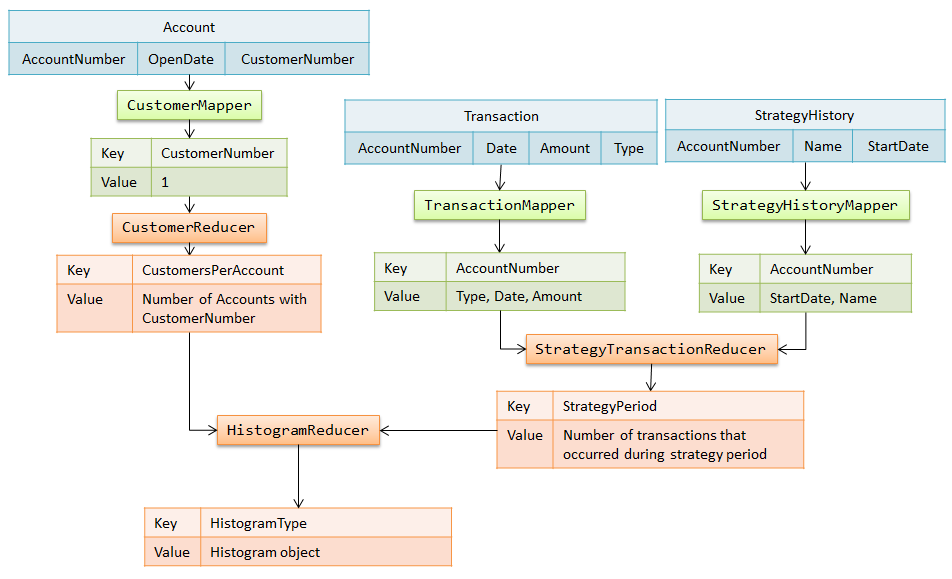
\includegraphics[scale=0.60]{../images/HistogramGen.png}
 % StageOne.png: 931x454 pixel, 96dpi, 24.64x12.01 cm, bb=0 0 698 341
  \caption{\texttt{HistogramGen} program flow diagram}
  \label{fig:histogen}
\end{figure}

The number of accounts per customer is determined by counting the number of \texttt{Account} entries with the same \texttt{CustomerNumber} attribute. This sum is found with the simple map and reduce methods shown below. The \texttt{CustomerMapper} takes each \texttt{Account} entry as input and maps the \texttt{CustomerNumber} for the account to a value of $1$. 
%   public static class CustomerMapper extends MapReduceBase 
%     implements Mapper<Object, Text, Text, IntWritable> 
%     {
%       public static final int COL_ACCOUNT_NUM = 0;
%       public static final int COL_OPEN_DATE = 1;
%       public static final int COL_CUSTOMER_NUM = 2;
%       public static final IntWritable ONE = new IntWritable(1);
% 
%       public void map(Object offset, Text input, 
%         OutputCollector<Text, IntWritable> output,
%         Reporter reporter) throws IOException 
%       {
%         String[] parts = (input.toString()).split(",");
%         String customerNumber = parts[COL_CUSTOMER_NUM].trim();
%         output.collect(new Text(customerNumber), ONE);
%       }
%   } 
{
\singlespace
\small
\begin{verbatim}
public void map(Object offset, Text input, 
     OutputCollector<Text, IntWritable> output, Reporter reporter) 
     throws IOException 
{
    String[] parts = (input.toString()).split(",");
    String customerNumber = parts[COL_CUSTOMER_NUM].trim();
    output.collect(new Text(customerNumber), ONE);
}
\end{verbatim}
}
The \texttt{CustomerReducer} receives the mapped output for each \texttt{CustomerNumber} key from the \texttt{CustomerMapper} and sums the value of each to get the total number of accounts for the \texttt{CustomerNumber} key. The resulting output is the total number of accounts for the customer mapped to the histogram type. 
%   public static class CustomerReducer extends MapReduceBase implements    
%     Reducer<Text, IntWritable, IntWritable, IntWritable> 
%   {
%     public static final IntWritable histogramType 
%             = new IntWritable(HistogramType.CUSTOMERS_PER_ACCOUNT.ordinal());
% 
%     public void reduce(Text customerNumber, Iterator<IntWritable> values,
%       OutputCollector<IntWritable, IntWritable> output,
%       Reporter reporter) throws IOException 
%     {
%       int count = 0;
%       while (values.hasNext())
%       {
%         count += values.next().get();
%       }
%       /* output the type of histogram and the count */
%       output.collect(histogramType, new IntWritable(count));
%     }
%   }
{
\singlespace
\small
\begin{verbatim}
public void reduce(Text customerNumber, Iterator<IntWritable> values,
      OutputCollector<IntWritable, IntWritable> output,
      Reporter reporter) throws IOException 
{
    int count = 0;
    while (values.hasNext())
    {
        count += values.next().get();
    }
    /* output the type of histogram and the count */
    output.collect(histogramType, new IntWritable(count));
}
\end{verbatim}
}

Furthermore, since performance depends on relationship complexity between the transaction data, the number of queries also depends on the strategy history and type of transaction for each strategy. Therefore, we evaluate the number of good standing and bad debt charges, adjustments, and payments per account. For each account, the number of transactions per strategy history are determined by counting the number of {\tt Transaction} entries with the same {\tt AccountNumber} attribute and the number of {\tt Transactions} that occur during each {\tt StrategyHistory} period. These sums are found with the simple map and reduce methods shown below. 

The {\tt TransactionMapper} maps the {\tt Transaction} to the owning {\tt AccountNumber}.
%  public static class TransactionMapper extends MapReduceBase implements 
%     Mapper<Object, Text, Text, ObjectWritable> 
%   {
%     public static final int COL_ACCOUNT_ID = 0;
%     public static final int COL_DATE = 1;
%     public static final int COL_AMOUNT = 2;
%     public static final int COL_TYPE = 3;
% 
%     public void map(Object offset, Text input,
%         OutputCollector<Text, ObjectWritable> output, Reporter reporter)
%         throws IOException 
%     {
%       String[] parts = input.toString().split(",");
%       String account = parts[COL_ACCOUNT_ID].trim();
%       String date = parts[COL_DATE].trim();
%       String amount = parts[COL_AMOUNT].trim();
%       String type = parts[COL_TYPE].trim();
% 
%       /* Output transactions by accountNumber */
%       Transaction transaction = new Transaction(date, type, amount);
%       output.collect(new Text(account), new ObjectWritable(transaction));
%     }
%   }
{
\singlespace
\small
\begin{verbatim}
public void map(Object offset, Text input, 
     OutputCollector<Text, ObjectWritable> output, Reporter reporter) 
     throws IOException 
{
    String[] parts = input.toString().split(",");
    String account = parts[COL_ACCOUNT_ID].trim();
    String date = parts[COL_DATE].trim();
    String amount = parts[COL_AMOUNT].trim();
    String type = parts[COL_TYPE].trim();

    /* Output transactions by accountNumber */
    Transaction transaction = new Transaction(date, type, amount);
    output.collect(new Text(account), new ObjectWritable(transaction));
}
\end{verbatim}
}
The {\tt StrategyMapper} maps the {\tt StrategyHistory} to the owning {\tt AccountNumber}.
%   public static class StrategyHistoryMapper extends MapReduceBase implements
%     Mapper<Object, Text, Text, ObjectWritable> 
%   {
%     public static final int COL_ACCOUNT_ID = 0;
%     public static final int COL_NAME = 1;
%     public static final int COL_DATE = 2;
% 
%     public void map(Object offset, Text input,
%       OutputCollector<Text, ObjectWritable> output, Reporter reporter)
%       throws IOException 
%     {
%       String[] parts = (input.toString()).split(",");
%       String account = parts[COL_ACCOUNT_ID].trim();
%       String name = parts[COL_NAME].trim();
%       String startDate = parts[COL_DATE].trim();
% 
%       /* Output strategy history by accountNumber */
%       StrategyHistory strategy = new StrategyHistory(startDate, name);
%       output.collect(new Text(account), new ObjectWritable(strategy));
%     }
%   }
{
\singlespace
\small
\begin{verbatim}
public void map(Object offset, Text input, 
    OutputCollector<Text, ObjectWritable> output, Reporter reporter)
    throws IOException 
{
    String[] parts = (input.toString()).split(",");
    String account = parts[COL_ACCOUNT_ID].trim();
    String name = parts[COL_NAME].trim();
    String startDate = parts[COL_DATE].trim();

    /* Output strategy history by accountNumber */
    StrategyHistory strategy = new StrategyHistory(startDate, name);
    output.collect(new Text(account), new ObjectWritable(strategy));
}
\end{verbatim}
}
The {\tt StrategyTransactionReducer} accepts key/value pairs from the\\ {\tt TransactionMapper} and {\tt StrategyHistoryMapper}, iterates through the list of events for the key account, and sums the values for each account. The output is the number of each transaction type per {\tt AccountNumber}.
{
\singlespace
\small
\begin{verbatim}
public void reduce(Text key, Iterator<ObjectWritable> values,
        OutputCollector<IntWritable, IntWritable> output, Reporter reporter)
        throws IOException 
{
    /* Keep list of payments */
    List<EventWritable> events = new ArrayList<EventWritable>();

    /* Keep track of strategy dates */
    Calendar goodStrategy = new GregorianCalendar();
    Calendar badDebt = new GregorianCalendar();

    while (values.hasNext()) 
    {
        EventWritable next = (EventWritable)        
        values.next().get();
        String type = next.getType().toString();
        events.add(next);
        /* Set good standing dates */
        if (type.equals(StrategyHistory.GOOD_STANDING)) 
        {
          //create event for 30, 60, 90 day after strategy starty date 
        }
        /* Set bad debt dates */
        else if (type.equals(StrategyHistory.BAD_DEBT)) 
        {
          //create event for 30, 60, 90 day after strategy starty date
        }
    }
        
    /* Sort by date and find sums */
    Collections.sort(events);
    for(EventWritable event : events) 
    {
        // count transactions per event strategy
    }

    // output one for each event strategy
    for(int i = 0; i < strategy_counts.length; i++)
    {
        output.collect(new IntWritable(i),newIntWritable(strategy_counts[i]));
    }
 }
\end{verbatim}
}

Finally, the {\tt HistogramReducer} consolidates the resulting output from the \\{\tt CustomerReducer} and {\tt StrategyTransactionReducer} into the final histogram.
{
\singlespace
\small
\begin{verbatim}
public void reduce(IntWritable key, Iterator<IntWritable> values,
        OutputCollector<Text, Histogram> output, Reporter reporter)
        throws IOException 
{
    /* What type of histogram is this? */
    HistogramType type = HistogramType.getType(key.get());

    /* add all the values to a temp list */
    ArrayList<Integer> temp = new ArrayList<Integer>();	
    while (values.hasNext()) 
    {
        temp.add(values.next().get());
    }

    /* sort list and create a new Histogram from data */
    Collections.sort(temp);
    Histogram histogram = new Histogram(type, temp.toArray(new Integer[0]));
    output.collect(new Text(type.toString()), histogram);
}
\end{verbatim}
}

\subsection{AccountGen: Test Data Generation}
The {\tt AccountGen} program uses the {\tt HistogramGen} probability distribution results to generate the test data sets with the {\tt Customer}, {\tt Account}, {\tt Transaction}, and {\tt StrategyHistory} entries. 

To decrease time requirements for generating large data sets, the work load is distributed among several mappers. For this, we define our own {\tt InputSplit} and {\tt RecordReader} to send an account number range to each mapper. Then for each account, the mapper uses the histogram statistics to determine:
\begin{enumerate}
 \item which {\tt CustomerNumber} to assign, and
 \item how many of each transaction type to generate (with the account number as the primary key).
\end{enumerate}

The {\tt MultipleOutputFormat} provided in the MapReduce API is used to output each entry (customer, account, transaction, strategy history) to a separate, comma-separated file. The attributes remain the same as the original entries. 

\section{MySQL Solution}
Since CompanyX already has a RDBMS implementation of the payment history analysis case study in place, we were able to leverage the existing SQL script used to pull expected results for the desired output file from tables in our MySQL solution. We developed the MySQL solution in the following steps:
\begin{enumerate}
 \item Define schema for payment history analysis database.
 \item Implement MySQL script to load account, customer, transaction and strategy history data into database tables.
 \item Update existing SQL script to execute in MySQL.
\end{enumerate}
We were able to derive the table definitions, data types, and constraints for the database schema from the provided background data and SQL query (see Appendix~\ref{app:mysql} for complete schema). Since we will be generating new data sets for each benchmark execution, we need to be able to dynamically load data into the MySQL database. Thus, we implemented a script to generate the MySQL load script based on a given input directory. The final load script is a series of statements of the following form-- \texttt{'load data local infile <filename>  into table <table name>'}. Finally, upon executing the SQL script in MySQL, we quickly realized that the existing SQL script used to pull expected results was not fully compatible with MySQL. So, the final step was to transform the incompatible queries to the MySQL standard and ensure that the result table matched the expected output table.

\section{Hadoop MapReduce Solution}
The MapReduce solution requires three map and reduce phases that are detailed in the following sections. 

\subsection{Stage 1: Customer Join Account}
The first stage combines the Customer and Account tables on the CustomerNumber using a \texttt{CustomerMapper}, \texttt{AccountMapper} and \texttt{CustomerJoinAccountReducer} (see Figure~\ref{fig:stage1}). 

\begin{figure}[hct]
% \begin{figure}[hct!]
 \centering
 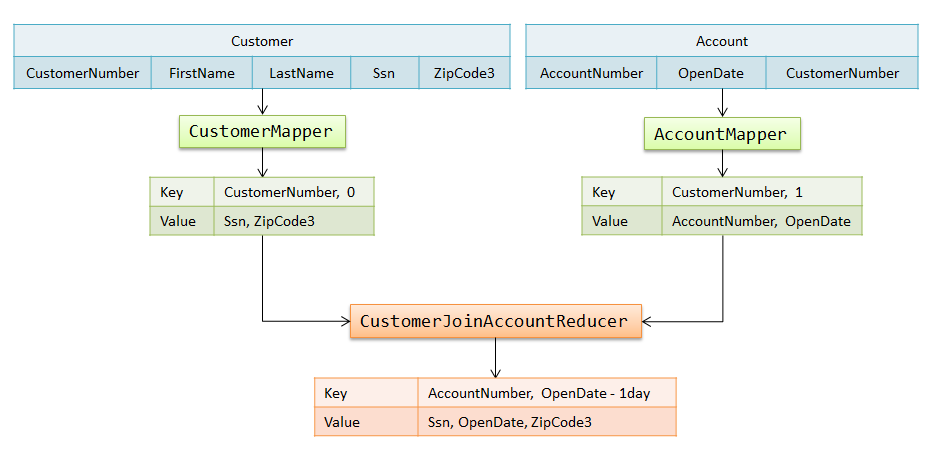
\includegraphics[scale=0.60,bb=0 0 698 341]{../images/StageOne.png}
 % StageOne.png: 931x454 pixel, 96dpi, 24.64x12.01 cm, bb=0 0 698 341
  \caption{Stage 1: Customer join Account program flow diagram}
  \label{fig:stage1}
\end{figure}

% \begin{description}
% \item[\textbf{Customer Mapper}]%\hspace*{\fill} \\
\subsubsection{Customer Mapper}
  \begin{itemize}
  \item The input is the \texttt{Customer} data (formatted as a .csv file). 
  \item The output key is \texttt{CustomerNumber} and the sort order for the key is \texttt{0}.
  \item The output value is \texttt{Ssn} and \texttt{ZipCode3} of the customer.
  \end{itemize}
{
\singlespace
\small
\begin{verbatim}
public void map(Object offset, Text input, 
    OutputCollector<TextPair, Text> output, Reporter reporter) 
    throws IOException {
    
    String[] parts = (input.toString()).split(",");

    String customerNumber = parts[COL_CUSTOMER_NUM].trim();
    String ssn = parts[COL_SSN].trim();
    String zipCode3 = parts[COL_ZIP_CODE_3].trim();

    key.set(new Text(customerNumber), ZERO);
    value = new Text(ssn + "," + zipCode3);

    output.collect(key, value);
}
\end{verbatim}
}
% \item[\textbf{Account Mapper}]\hspace*{\fill} \\
\subsubsection{Account Mapper}
  \begin{itemize}
  \item The input is the \texttt{Account} data (formatted as a .csv file).
  \item The output key is \texttt{CustomerNumber} and the sort order for the key is \texttt{1}.
  \item The output value is \texttt{AccountNumber} and \texttt{OpenDate} of the account.
  \end{itemize}
{
\singlespace
\small
\begin{verbatim}
public void map(Object offset, Text input,
    OutputCollector<TextPair, Text> output, Reporter reporter) 
    throws IOException {

    String[] parts = (input.toString()).split(",");

    String accountNumber = parts[COL_ACCOUNT_NUM].trim();
    String openDate = parts[COL_OPEN_DATE].trim();
    String customerNumber = parts[COL_CUSTOMER_NUM].trim();

    key.set(customerNumber, "1");
    value = new Text(accountNumber + "," + openDate);
    output.collect(key, value);
}
\end{verbatim}
}
% \item[\textbf{Customer JOIN Account Reducer}]\hspace*{\fill} \\
\subsubsection{Customer Join Account Reducer}
  \begin{itemize}
  \item The input is the sorted output from the Customer and Account mappers. Since the key value of each Customer is unique and the sort order for the
  Customer is 0, the Customer will be the first input value followed by a list of Accounts owned by the Customer. 
  \item The output key is \texttt{AccountNumber} and the sort order for the key is \texttt{OpenDate}.
  \item The output value is
    \begin{itemize}
	 \item \texttt{Ssn},
	 \item \texttt{OpenDate}, and
	 \item \texttt{ZipCode3}.
    \end{itemize}
  \end{itemize}
% \end{description}

\subsection{Stage 2: Strategy History Join Transaction}
The second stage combines the Account and Customer data from stage 1 and the Strategy History and Transaction tables on the AccountNumber. This process requires the output from stage one and a \texttt{StrategyHistoryMapper}, \texttt{TransactionMapper} and\\ \texttt{CustomerJoinAccountReducer} (see Figure~\ref{fig:stage2}). 

\begin{figure}[htc!]
 \centering
 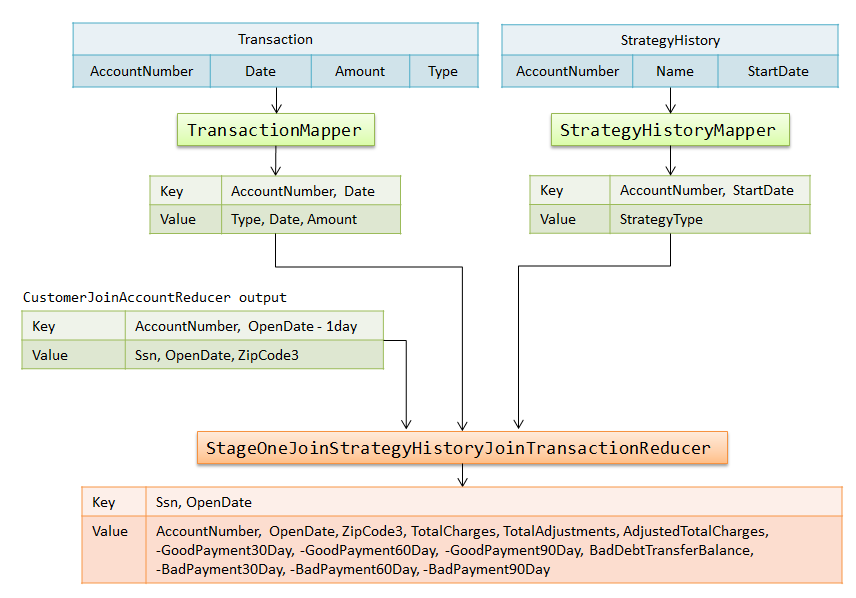
\includegraphics[scale=0.60,bb=0 0 698 341]{../images/StageTwo.png}
 % StageOne.png: 931x454 pixel, 96dpi, 24.64x12.01 cm, bb=0 0 698 341
  \caption{Stage 2: Stragety History join Transaction program flow diagram}
  \label{fig:stage2}
\end{figure}

\subsubsection{Strategy History Mapper}
\begin{itemize}
 \item The input is the \texttt{Strategy History} data (formatted as a .csv
file).
 \item The output key is \texttt{AccountNumber} and the sort order for the key is \texttt{StrategyStartDate}.
 \item The output value is \texttt{StrategyName} of the strategy history. 
\end{itemize}
Note that multiple key/value pairs are output from this mapper. The pair for the strategy start date is output followed by a pair for each of thirty, sixty, and ninety days after the strategy start date.

{
\singlespace
\small
\begin{verbatim}
public void map(Object offset, Text input, 
    OutputCollector<TextDatePair, Text> output, Reporter reporter) 
    throws IOException {

    String[] parts = (input.toString()).split(",");

    String accountNumber = parts[COL_ACCOUNT_NUMBER].trim();
    String name = parts[COL_NAME].trim();
    int type = StrategyType.getByName(name).getNumberOfDays();

    calendar.setTime(DateWritable.df.parse(parts[COL_DATE].trim()));

    key.set(accountNumber, calendar.getTime());
    value.set(Integer.toString(type));
    output.collect(key, value);

    calendar.add(Calendar.DAY_OF_MONTH, 30);
    key.set(accountNumber, calendar.getTime());
    value.set(Integer.toString(type + 1));
    output.collect(key, value);

    calendar.add(Calendar.DAY_OF_MONTH, 30);
    key.set(accountNumber, calendar.getTime());
    value.set(Integer.toString(type + 2));
    output.collect(key, value);

    calendar.add(Calendar.DAY_OF_MONTH, 30);
    key.set(accountNumber, calendar.getTime());
    value.set(Integer.toString(type + 3));
    output.collect(key, value);
}
\end{verbatim}
}

\subsubsection{Transaction Mapper}
\begin{itemize}
 \item The input is the \texttt{Transaction} data (formatted as a .csv file).
 \item The output key is \texttt{AccountNumber} and the sort order for the key is \texttt{TransactionDate}.
 \item The output value is
  \begin{itemize}
    \item \texttt{TransactionType},
    \item \texttt{TransactionDate}, and
    \item \texttt{TransactionAmount} of the transaction.
  \end{itemize}
\end{itemize}.
{
\singlespace
\small
\begin{verbatim}
public void map(Object offset, Text input, 
    OutputCollector<TextDatePair, Text> output, Reporter reporter) 
    throws IOException {

    String[] parts = input.toString().split(",");

    String accountNumber = parts[COL_ACCOUNT_ID].trim();
    String date = parts[COL_DATE].trim();
    String amount = parts[COL_AMOUNT].trim();
    int type = TransactionType.getByName(parts[COL_TYPE].trim()).getOffset();

    key.set(accountNumber, date);
    value.set(type + "," + date + "," + amount);

    output.collect(key, value);
}
\end{verbatim}
}
\subsubsection{Strategy History Join Transaction Reducer}
\begin{itemize}
 \item The input is the sorted output from phase 1 and the Strategy History and
Transaction mappers. Since the output from phase 1 is sorted by the
OpenDate of the Account, it will always be first (because the account must
be opened before any Strategy History or Transactions exist). Also, the key of
each Strategy History is unique and the sort order for both the Strategy History
and Transaction values are by date, so the Transaction values will be separated
into each strategy time period (thirty, sixty, and ninety day) by the Strategy
History values.
 \item The output key is \texttt{Ssn} and the sort order for the key is \texttt{OpenDate}.
 \item The output value is
  \begin{itemize}
  \item \texttt{AccountNumber},
  \item \texttt{OpenDate},
  \item \texttt{ZipCode3},
  \item \texttt{TotalCharges},
  \item \texttt{TotalAdjustments},
  \item \texttt{AdjustedTotalCharges},
  \item \texttt{TotalGoodStandingPayments30Day},
  \item \texttt{TotalGoodStandingPayments60Day},
  \item \texttt{TotalGoodStandingPayments90Day},
  \item  \texttt{BadDebtTransferBalance},
  \item \texttt{TotalBadDebtPayments30Day}, 
  \item \texttt{TotalBadDebtPayments60Day}, and
  \item \texttt{TotalBadDebtPayments90Day}.
  \end{itemize}
\end{itemize}

\subsection{Stage 3: Combine Results}
The final stage uses the output from stage 2 to gather the previous account data for each account (see Figure~\ref{fig:stage3}).

\begin{figure}[htc!]
 \centering
 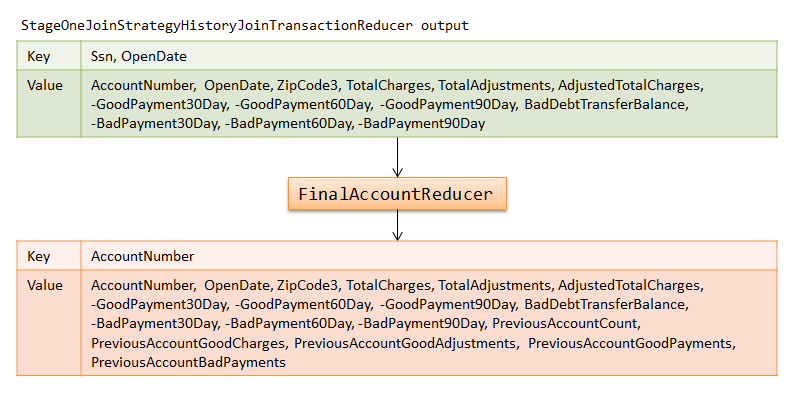
\includegraphics[scale=0.60,bb=0 0 698 341]{../images/StageThree.png}
 % StageOne.png: 931x454 pixel, 96dpi, 24.64x12.01 cm, bb=0 0 698 341
 \caption{Stage 3: Combine results program flow diagram}
 \label{fig:stage3}
\end{figure}

\subsubsection{Identity Mapper}
\begin{itemize}
 \item The input is the sorted output from stage 2. 
 \item The output key is \texttt{AccountNumber}.
 \item The output value is the output value from stage 2 followed by 
   \begin{itemize}
    \item \texttt{PreviousAccountCount},
    \item \texttt{PreviousAccountGoodStandingCharges},
    \item \texttt{PreviousAccountGoodStandingAdjustments},
    \item \texttt{PreviousAccountGoodStandingPayments}, and
    \item \texttt{PreviousAccountBadDebtPayments}.
    \end{itemize}
\end{itemize}

\section{Hive Solution}
Because the HQL syntax is similar to the SQL syntax, we could also leverage CompanyX's existing SQL script for our Hive solution. Similar to the MySQL solution, the steps required for this implementation are:

\begin{enumerate}
 \item Define schema for payment history analysis database.
 \item Implement HQL script to load account, customer, transaction and strategy history data into database tables.
 \item Transform existing SQL script to HQL for Hive execution.
\end{enumerate}

In our case, the major difference between the Hive and MySQL database schema is the additional \texttt{CLUSTERED BY} parameter provided for each table definition. For each table defined in the schema, we cluster by the primary key column into 4 buckets. As in the MySQL solution, we dynamically generate the HQL load script based on a given input directory. The final load script is a series of statements of the following form-- \texttt{'load data inpath <filename> into table <table name>'}. The HQL database schema can be found in Appendix~\ref{app:hive}. 
%%%%%%%%%%%%%%%%%%%%%%%%%%%%%%%%%%%%%%%%%%%%%%%%%%%%%%%%%%%%%%%%%%%%%%%%%%%%%%
%
% Chapter: Results and Conclusions
%
%%%%%%%%%%%%%%%%%%%%%%%%%%%%%%%%%%%%%%%%%%%%%%%%%%%%%%%%%%%%%%%%%%%%%%%%%%%%%%
%%%%%%%%%%%%%%%%%%%%%%%%%%%%%%%%%%%%%%%%%%%%%%%%%%%%%%%%%%%%%%%%%%%%%%%%%% % %
%
% Chapter: Results and Conclusions
% Experimental and/or Theoretical Results demonstrating/proving your solution 
% This section should thoroughly describe the results you obtained. Whenever 
% possible or appropriate, you should try to present your results pictorially 
% using graphs or histograms. In addition you must explain your results; tell 
% the reader what all these data mean.
% Explain the tests you performed (and why)
% Explain how you gathered the data and describe the environment in which you 
% gathered data (include description of any simplifying assumptions you made, 
% any software you wrote or used to run your experiments)
% Present your results. Choose quality over quantity; the reader will not be 
% impressed with pages and pages of graphs and tables, instead s/he wants to 
% be convinced that your results show something interesting and that your 
% experiments support your conclusions.
% Discuss your results! Explain and interpret your results (possibly compare 
% your results to related work). Do not just present data and leave it up to 
% the reader to infer what the data show and why they are interesting. 
% Negative results are interesting too; don't try to hide bad results, but 
% do try to explain them.
%
%%%%%%%%%%%%%%%%%%%%%%%%%%%%%%%%%%%%%%%%%%%%%%%%%%%%%%%%%%%%%%%%%%%%%%%%%%%%%%
 
\chapter{Experimental Results and Analysis: MySQL, MapReduce, and Hive Performance Comparison} \label{ch:results}
This chapter details the RDBMS and DDMS performance comparison experiment using our solutions to the payment history analysis case study. For each solution, we discuss the efficiency and scalability, along with the resulting implications for SMB data management. Our goal was to determine at what point Hadoop and Hive would out-perform MySQL.

The experiment was conducted on the Boise State University Onyx cluster. The cluster configuration and detailed hardware specifications are provided in Appendix~\ref{app:cluster-config}. The experiment was executed sequentially to ensure exclusive access to the server and cluster resources and to avoid the overhead of parallel task execution. Before each execution, we ensured that all nodes were alive and that the integrity of the data was unaltered. Each of the run-times reported reflects the average of three program executions.

\section{Setup}
To provide a fair and controlled environment for our benchmark analysis, we needed to ensure that the computing power of the distributed systems running Hadoop and Hive were comparable to the system running MySQL. 

We installed MySQL on the master node (node00) of the Onyx cluster which is a 4-core hyper-threaded processor, yielding a total of 8 processing threads. We installed the version 5.1.48 (x86\_64) of the MySQL Community Server release for redhat-linux-gnu on the master node of Onyx. The system was configured to use 16GB for the max allowed packet size and 16MB for the net buffer length. We deleted the tables and reloaded the data for each experiment to ensure that the queries were not stored in memory.

We installed Hadoop version 0.20.2 running on Java 1.6.0\_21 which includes both the HDFS and Mapreduce in both pseudo-distributed and distributed configurations. First, we configured the HDFS namenode and MapReduce JobTracker on the Onyx master node (the same as the MySQL server) along with 4 compute nodes as HDFS datanodes and MapReduce TaskTrackers-- also yielding a total of 8 processing threads. Note that since the purpose of the namenode is to maintain the filesystem tree, the metadata for directories in the tree, and the datanode on which all the blocks for a given file are located~\cite{white}, it does not add computing power for MapReduce or Hive in this experiment. We set the number of map tasks per job (\textit{mapred.map.tasks}) to 8, which is 1 task per core. The maximum number of map and reduce tasks are set to 16 and 17, respectively. We left the default replication factor of 3 per block, without compression. Data for both the namenode and datanodes are stored on an \texttt{ext4} directory of the local filesystem. Then, to test Hadoop on the exact same hardware as MySQL, we configured Hadoop to run in pseudo-distributed mode on the master node. In pseudo-distributed mode, each Hadoop daemon runs in a separate Java process. After each benchmark test, we destroy and reformat the HDFS to ensure the uniform distribution of data across nodes. 

We installed Hive version 0.7.0 and configured it to run on top of the same HDFS instance described above. To increase performance, we cluster the tables by primary key into buckets and store data in row format.

\section{Execution}
To determine how well each approach scales as the amount of data increases, we executed the performance benchmark on small (200MB to 500MB), medium (1GB to 5GB), and large (5GB to 10GB) data set sizes. Thus, we varied the number of accounts in the payment analysis data set from 500 to 20,000 records. Each trial was executed from a single client on the master node.

We implemented a performance benchmark test suite using bash shell scripting to help automate the execution process. The suite includes a performance benchmark executable for each of the three solutions that perform the steps enumerated below.

\begin{itemize}
 \item \textbf{MySQL}-- (1) load payment schema to MySQL database, (2) extract data from HDFS using FUSE-DFS module and load to MySQL database tables, (3) execute payment history analysis query, and (4) append query run-time to performance result file.
 \item \textbf{MapReduce}-- (1) ensure HDFS status, (2) execute payment history analysis program, and (3) append program run-time to performance result file.
 \item \textbf{Hive}-- (1) load payment schema to Hive database, (2) load data from HDFS to the Hive database, (3) execute HiveQL payment history analysis query, and (4) append query run-time to performance result file.
\end{itemize}

The suite also includes a script to sequentially run all of the above test scripts for each each trial size, where the experiment procedure is as follows:
\begin{enumerate}
 \item Generate the test data set using \texttt{AccountGen} for the given trial size and record the size of the data set in the performance result file. (On first run, this also involves executing \texttt{HistogramGen} to input for \texttt{AccountGen}).
 \item Execute the MapReduce performance benchmark.
 \item Execute the MySQL performance benchmark.
 \item Execute the Hive performance benchmark.
\end{enumerate}

\section{Results}
Since we chose to generate data based on the number of accounts, we provide the approximate size of the generated data set, namely the \textit{trial size}, for each number of accounts used in our experiments in Table~\ref{tbl:datasetsize}. The approximate sizes are an average of generated data from each of the three trial runs.

 \begin{table}[ht]
  \caption{ Approximate trial size of data set for number of Account records }
  \label{tbl:datasetsize}
  \centerline{
  \small
  \begin{tabular}{|l|l|}
   \hline
   \# Accounts & Approximate trial size\\[0.5ex]
   \hline\hline
   500 & 235 MB\\
   \hline
   1000 & 475 MB\\
   \hline
   2500 & 1 GB\\
   \hline
   5000 & 2 GB\\
   \hline
   10000 & 5 GB\\
   \hline
   15000 & 7 GB\\
   \hline
   20000 & 9 GB\\
   \hline
  \end{tabular}
  }
 \end{table}

Figure~\ref{fig:allruntimes} and Table~\ref{tbl:results} display the performance results of MySQL, MapReduce and Hive for each trial size with the MySQL server running on the master node of the onyx cluster and the Hadoop namenode running on the master node of the Onyx cluster and four data nodes running on four compute nodes.  

 \begin{table}[ht]
  \caption{Run-time (seconds) performance of MySQL server running on master node and MapReduce / Hive running on master node plus four data nodes}
  \label{tbl:results}
  \centerline{
  \small
  \begin{tabular}{|l||l|l|l|}
   \hline
   \# Accounts& MySQL & MapReduce & Hive\\[0.5ex]
   \hline\hline
   500 & 4.20 & 81.14 & 535.1\\
   \hline
   1000 & 13.83 & 82.55 & 543.64\\
   \hline
   2500 & 85.42 & 84.41 & 548.45\\
   \hline
   5000 & 392.42 & 83.42 & 553.44\\
   \hline
   10000 & 1518.18 & 88.14 & 557.51\\
   \hline
   15000 & 1390.25 & 86.85 & 581.5\\
   \hline
   20000 & 2367.81 & 88.90 & 582.7\\
   \hline
  \end{tabular}
  }
 \end{table}

\begin{figure}[h!]
 \centering
 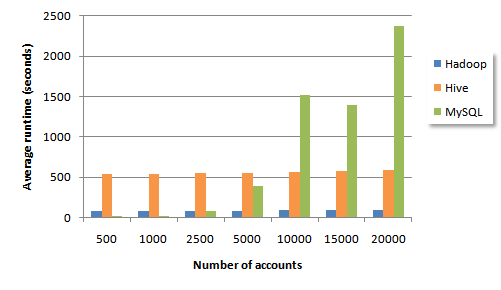
\includegraphics[width=\textwidth]{../images/runtime_vs_accountCount.png}
 % graph-all-runtimes.eps: 0x0 pixel, 300dpi, 0.00x0.00 cm, bb=14 14 630 433
 \caption{Run-time (seconds) performance of MySQL server running on master node and MapReduce / Hive running on master node plus four data nodes}
 \label{fig:allruntimes}
\end{figure}

Figure~\ref{fig:allruntimespseudo} and Table~\ref{tbl:resultspseudo} display the performance results of MySQL, MapReduce and Hive for each trial size with MySQL server running on the master node of the Onyx cluster and Hadoop running in pseudo-distributed mode on the master node of the Onyx cluster.  

 \begin{table}[ht]
  \caption{Run-time (seconds) performance of MySQL server running on master node and MapReduce / Hive running in pseudo-distributed mode}
  \label{tbl:resultspseudo}
  \centerline{
  \small
  \begin{tabular}{|l||l|l|l|}
   \hline
   \# Accounts& MySQL & MapReduce & Hive\\[0.5ex]
   \hline\hline
   500 & 4.20 & 79.45 & 532.01\\
   \hline
   1000 & 13.83 & 79.50 & 531.55\\
   \hline
   2500 & 85.42 & 79.42 & 534.16\\
   \hline
   5000 & 392.42 & 79.44 & 537.00\\
   \hline
   10000 & 1518.18 & 81.48 & 543.51\\
   \hline
   15000 & 1390.25 & 82.39 & 543.95\\
   \hline
   20000 & 2367.81 & 87.47 & 543.64\\
   \hline
  \end{tabular}
  }
 \end{table}

\begin{figure}[h!]
 \centering
 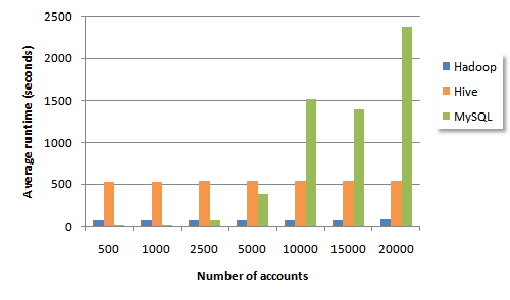
\includegraphics[width=\textwidth]{../images/runtime_vs_accountCount_pseudoDistributed.png}
 % graph-all-runtimes.eps: 0x0 pixel, 300dpi, 0.00x0.00 cm, bb=14 14 630 433
 \caption{Run-time (seconds) performance of MySQL server running on master node and MapReduce / Hive running on master node in pseudo-distributed mode}
 \label{fig:allruntimespseudo}
\end{figure}

MySQL outperforms both MapReduce and Hive for trial sizes ranging from 500 to 2,500 accounts. Since the amount of data generated for these trials is relatively small, 235MB to 1GB, the results are as expected. Aside from an anomaly at 15,000 accounts, the run-times continue to increase as expected with the size of the data set. At 15,000 accounts the MySQL run-time decreases from 1518.18 seconds to 1390.25 seconds. The MapReduce run-time also decreases from 88.14 seconds to 86.85 seconds at this same trial size. Since the data is randomly generated and the anomaly occurred for both MySQL and Hive, it may be explained by less complex data in this data range.

In both distributed and pseudo-distributed mode, MapReduce run-times remain steady at in the range of 81 to 90 seconds for all trial sizes, converging and surpassing MySQL performance at around 2,500 accounts. Hive run-times also remain steady in the range of 535 to 583 seconds for all trials, converging and surpassing MySQL performance at around 5,000 accounts. As expected with the relatively small trial sizes, MapReduce and Hive performed better in psuedo-distributed mode than in distributed mode with the same number of processing cores because there is no network communication and the drives are twice as fast. However, as the amount of data increases we expect better performance in distributed mode.

%  \begin{table}[ht]
%   \caption{The average run-times (seconds) per account}
%   \label{tbl:avg-account-runtimes}
%   \centerline{
%   \small
%   \begin{tabular}{|l||l|l|l|}
%    \hline
%    \# Accounts & MySQL & MapReduce & Hive\\[0.5ex]
%    \hline\hline
%    500 & 0.01 & 0.16 & 1.07\\
%    \hline
%    1000 & 0.01 & 0.08 & 0.54\\
%    \hline
%    2500 & 0.03 & 0.03 & 0.22\\
%    \hline
%    5000 & 0.08 & 0.02 & 0.11\\
%    \hline
%    10000 & 0.15 & 0.01 & 0.06\\
%    \hline
%    15000 & 0.09 & 0.01 & 0.04\\
%    \hline
%    20000 & 0.12 & 0 & 0.03\\
%    \hline
%   \end{tabular}
%   }
%  \end{table}
% 
% Table ~\ref{tbl:avg-account-runtimes} displays the solution run-times divided by the trial size. It is evident that performance per account for both MapReduce and Hive improves as the trial size increases, whereas the MySQL performance decreases. 

From these results, it is evident that MapReduce outperforms MySQL and Hive by a dramatic margin. Therefore, for test data sets greater than 1GB, MapReduce emerges as the best candidate solution for the payment history analysis case study provided by CompanyX. Furthermore, we investigate whether we can improve MapReduce performance further by varying the number of map tasks per datanode; Figure ~\ref{fig:maptasks} displays the results for 1, 2, and 4 map tasks per datanode. In this case, we observe that MapReduce with 1 map task per datanode slightly outperforms 2 and 4 map tasks per datanode.

\begin{figure}[h!]
 \centering
 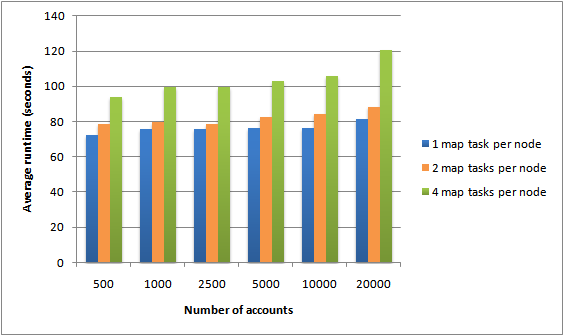
\includegraphics[width=\textwidth]{../images/runtime_vs_mapTasks.png}
 % graph-all-runtimes.eps: 0x0 pixel, 300dpi, 0.00x0.00 cm, bb=14 14 630 433
 \caption{Scalability of MapReduce run-time (seconds) performance for a varied number of map tasks per datanode}
 \label{fig:maptasks}
\end{figure}
%%%%%%%%%%%%%%%%%%%%%%%%%%%%%%%%%%%%%%%%%%%%%%%%%%%%%%%%%%%%%%%%%%%%%%%%%%%%%%
%
% Chapter: Conclusion
%
%%%%%%%%%%%%%%%%%%%%%%%%%%%%%%%%%%%%%%%%%%%%%%%%%%%%%%%%%%%%%%%%%%%%%%%%%%%%%%
%%%%%%%%%%%%%%%%%%%%%%%%%%%%%%%%%%%%%%%%%%%%%%%%%%%%%%%%%%%%%%%%%%%%%%%%%%%%%%
%
% Chapter: Conclusion
%
%%%%%%%%%%%%%%%%%%%%%%%%%%%%%%%%%%%%%%%%%%%%%%%%%%%%%%%%%%%%%%%%%%%%%%%%%%%%%%
 
\chapter{Conclusion} \label{ch:conclusion}
In this chapter we conclude by summarizing our findings, listing implications and suggesting future directions for CompanyX.

\section{Summary}
In Chapter ~\ref{ch:intro} we started by introducing the concepts of this research project. We provided brief summary of BI, listed various data access and storage obstacles for SMBs, and highlighted the importance of conducting this OSS database management investigation.

In Chapter~\ref{ch:background} we provided a background for concepts pertaining to BI storage, access, and analytical systems. Here, we outlined some major challenges faced by SMBs interested in BI analytics and discuss RDBMS and alternative DDBMS solutions. We summarized the notion of Big Data, a likely future obstacle for the SMB, and provided relevant information regarding the Hadoop solutions considered in this research: MapReduce and Hive.

In Chapter~\ref{ch:problem} we introduced the payment history analysis case study for a specific SMB. We explained how this particular SMB designs software tools to analyze current and historical payment habits on customer data and attempts forecast trends. We discussed the database management challenges faced by the SMB as their customer base expands and defined their specific case study. Here, we explained their data storage and access models, along with the requisite test data set generation utilities required to conduct the analysis. In doing so, we formally presented the problem statement and list the inquiries we wish to address in this research project.

In Chapter~\ref{ch:solution} we defined the design and implementation for the RDBMS and DDBMS solutions. First, we discussed the detailed process of generating the test data set and provided a summarized description of the key algorithms and data structures employed by these utilities: the \texttt{HistogramGen} and \texttt{AccountGen} MapReduce programs. Second, we discussed the central components of the MySQL, Hadoop MapReduce, and Hadoop Hive solution implementation, where we explained the process by which they are used to instrument the payment history analysis case study (as presented in Chapter~\ref{ch:problem}).

In Chapter~\ref{ch:results} we detailed the RDBMS and DDMS performance comparison experiment (for the solutions of Chapter~\ref{ch:solution}). Here, we discussed the efficiency and scalability for these implementations, along with the resulting implications and analysis for this SMB's data management case study (as expressed in Chapter~\ref{ch:problem}). First, we discussed the software and hardware environment in which our comparative benchmark analysis is conducted. Second, we provided the procedure used to guide and execute the experiment. Finally, we presented the performance results for the various experimental trial runs: to summarize, we observed that the MapReduce solution outperforms its competitors for the case study.

\section{Results and Implications}
From the payment history analysis performance comparison between MySQL, MapReduce and Hive, we conclude that:

\begin{enumerate}
  \item MySQL performs the best for trial sizes ranging from 500 to 2,500 accounts, but does not scale well beyond that,
  \item Hive performance remained constant for all trial sizes, matching and surpassing MySQL performance at 5,000 accounts,
  \item MapReduce outperformed Hive and remained constant for all trial sizes, matching and surpassing MySQL at 2,500 accounts.
\end{enumerate}

Our results indicate that MapReduce is the best candidate for this case study. Therefore, we recommend that CompanyX deploy this type of distributed warehousing solution for their BI predictive analytics. 

\section{Future Direction}
Beyond the scope of this project, it would be interesting to investigate RDBMS and DDMS implementations further. 

\begin{itemize}
 \item \textbf{RDBMS}
  \begin{enumerate}
   \item Benchmark performance of several RDBMS implementations including MySQL Enterprise edition, Microsoft SQLServer, PostresQL, and Oracle.
   \item Investigate the performance ratio of parallel database solutions.
  \end{enumerate}
 \item \textbf{DDMS}
  \begin{enumerate}
   \item MapReduce-- test on several cluster environments, implement and compare performance on varied account complexity
   \item Hive-- perform payment analysis benchmarks on various cluster configurations and account data
  \end{enumerate}
\end{itemize}

\backmatter

%%%%%%%%%%%%%%%%%%%%%%%%%%%%%%%%%%%%%%%%%%%%%%%%%%%%%%%%%%%%%%%%%%%%%%%%%%%%%%
%
% Bibilography
%
%%%%%%%%%%%%%%%%%%%%%%%%%%%%%%%%%%%%%%%%%%%%%%%%%%%%%%%%%%%%%%%%%%%%%%%%%%%%%%

% There are different bibliography styles; 'plain' is used for theses.
\bibliographystyle{plain}
\bibliography{marissa-hollingsworth-project}

%%%%%%%%%%%%%%%%%%%%%%%%%%%%%%%%%%%%%%%%%%%%%%%%%%%%%%%%%%%%%%%%%%%%%%%%%%%%%%
%
% Appendix
%
%%%%%%%%%%%%%%%%%%%%%%%%%%%%%%%%%%%%%%%%%%%%%%%%%%%%%%%%%%%%%%%%%%%%%%%%%%%%%%
\appendix

%%%%%%%%%%%%%%%%%%%%%%%%%%%%%%%%%%%%%%%%%%%%%%%%%%%%%%%%%%%%%%%%%%%%%%%%%%%%%%
%
% Appendix: Data Model
%
%%%%%%%%%%%%%%%%%%%%%%%%%%%%%%%%%%%%%%%%%%%%%%%%%%%%%%%%%%%%%%%%%%%%%%%%%%%%%%
\chapter{MySQL Payment History Database Schema} \label{app:mysql}
\begin{figure}[hct]
% \begin{figure}[hct!]
 \centering
 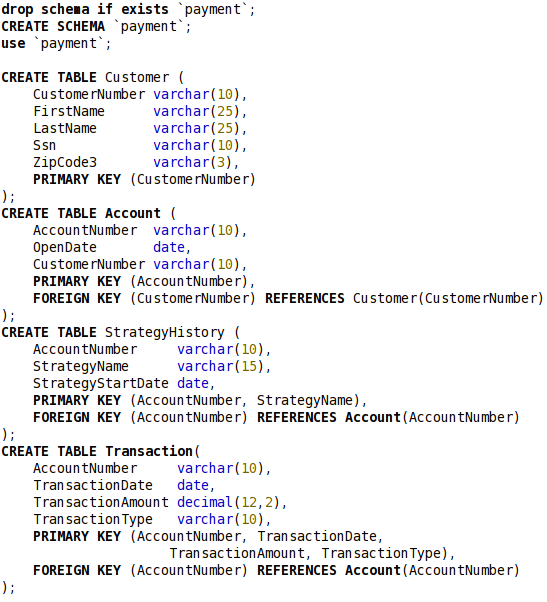
\includegraphics[scale=0.90]{../images/sql_payment_schema.png}
%  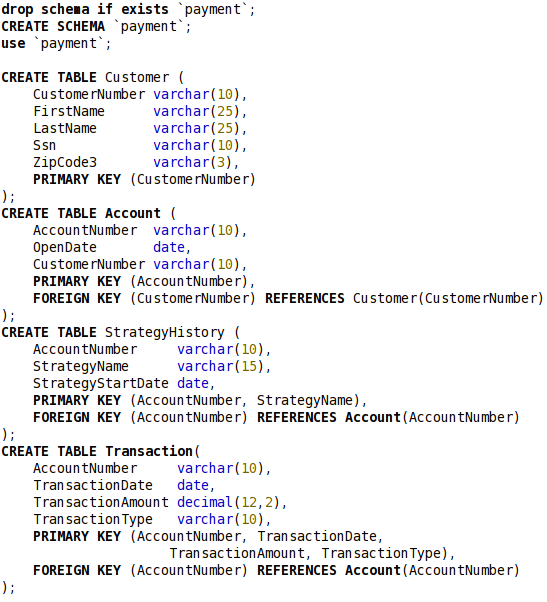
\includegraphics[scale=0.60,bb=0 0 698 341]{../images/sql_payment_schema.png}
 % StageOne.png: 931x454 pixel, 96dpi, 24.64x12.01 cm, bb=0 0 698 341
\end{figure}

%%%%%%%%%%%%%%%%%%%%%%%%%%%%%%%%%%%%%%%%%%%%%%%%%%%%%%%%%%%%%%%%%%%%%%%%%%%%%%
%
% Appendix: Cluster Configuration
%
%%%%%%%%%%%%%%%%%%%%%%%%%%%%%%%%%%%%%%%%%%%%%%%%%%%%%%%%%%%%%%%%%%%%%%%%%%%%%%
\chapter{Cluster Configuration} \label{app:cluster-config}
The benchmark experiments for MySQL, MapReduce and Hive were executed on the
College of Engineering, Department of Computer Science, Onyx cluster at Boise
State University. The cluster has one master node (node00) and 32 compute nodes (node01-node32), 
which are connected with a private Broadcom Corporation NetXtreme BCM5754 Gigabit
Ethernet switch. Figure~\ref{fig:linux-cluster} shows the layout of the Onyx cluster lab.

\begin{figure}[h!]
 \centering
 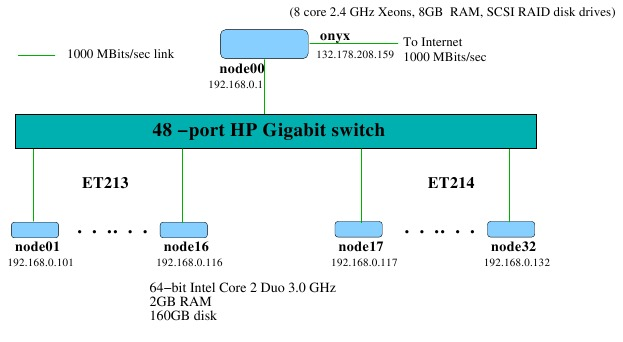
\includegraphics[bb=0 0 477 262]{../images/linux-cluster-lab.jpg}
 % linux-cluster-lab.jpg: 623x342 pixel, 94dpi, 16.84x9.24 cm, bb=0 0 477 262
 \caption{Boise State University, Department of Computer Science, Onyx Cluster Lab}
\label{fig:linux-cluster}
\end{figure}

Master node (node00) is an Intel(R) Xeon(R) E5530 @ 2.40GHz processor with
hyper-threading. It has a total of 8 processing threads (4 cores with 2 threads
per core) and 15K RPM SCSI drives with RAID-6.

Each compute node (node01-node32) is an Intel(R) Core(TM)2 Duo E8400 @ 3.00GHz
processor with 2 threads per node (2 cores with 1 thread per core). Each
compute node has a 7200 RPM SATA disk drive.

%%%%%%%%%%%%%%%%%%%%%%%%%%%%%%%%%%%%%%%%%%%%%%%%%%%%%%%%%%%%%%%%%%%%%%%%%%%%%%
%
% Appendix: Data Model
%
%%%%%%%%%%%%%%%%%%%%%%%%%%%%%%%%%%%%%%%%%%%%%%%%%%%%%%%%%%%%%%%%%%%%%%%%%%%%%%
\chapter{Hive Payment History Database Schema} \label{app:hive}
\begin{figure}[hct]
% \begin{figure}[hct!]
 \centering
 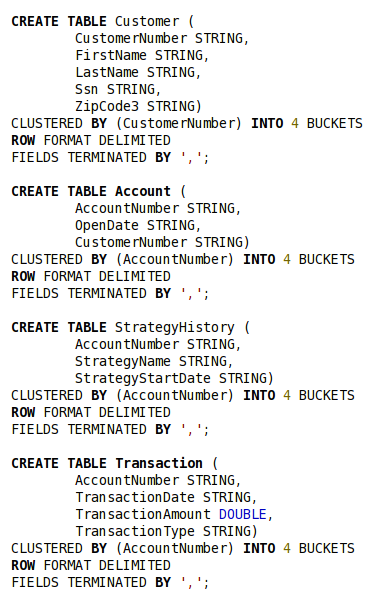
\includegraphics[scale=0.90]{../images/hive_payment_schema.png}
%  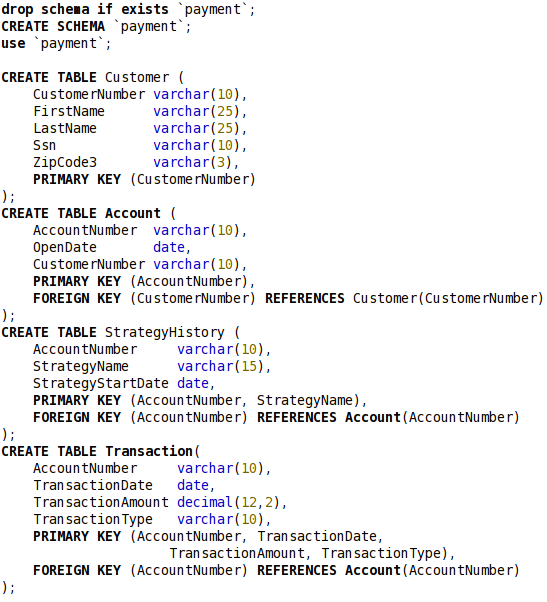
\includegraphics[scale=0.60,bb=0 0 698 341]{../images/sql_payment_schema.png}
 % StageOne.png: 931x454 pixel, 96dpi, 24.64x12.01 cm, bb=0 0 698 341
\end{figure}



\finish  %! Do not remove!

\end{document}
